% *********************************************************************
% © 2021–2026 Jeremy Sylvestre
%
% Permission is granted to copy, distribute and/or modify this document
% under the terms of the GNU Free Documentation License, Version 1.3 or
% any later version published by the Free Software Foundation; with no
% Invariant Sections, no Front-Cover Texts, and no Back-Cover Texts. A
% copy of the license is included in the appendix entitled “GNU Free
% Documentation License” that appears in the output document of this
% PreTeXt source code. All trademarks™ are the registered® marks of
% their respective owners.
%
% *********************************************************************

\newcommand*{\xmin}{2.985}
\newcommand*{\xmax}{3.015}
\newcommand*{\ymin}{3.735}
\newcommand*{\ymax}{3.765}
\newcommand*{\func}{\x * \x * \x * \x / 4 - 3 * \x * \x * \x + 23 * \x * \x / 2 - 14 * \x + 3}

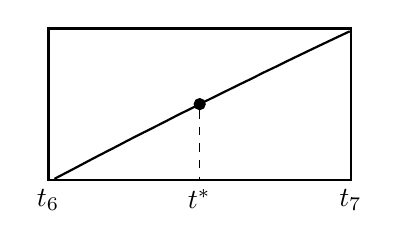
\begin{tikzpicture}
[
	closedpt/.style={circle,draw,fill,inner sep=0pt,minimum size=4pt},
	openpt/.style={circle,draw,inner sep=0pt,minimum size=4pt},
	xscale=128,
	yscale=64
]

	\draw[thick] (\xmin,\ymin) rectangle (\xmax,\ymax);
	\node[below] at (\xmin,\ymin) {$t_6$};
	\node[below] at (\xmax,\ymin) {$t_7$};

	% example graph
	\draw[thick, domain=2.9856:3.0151, smooth, thick] plot (\x,{\func});

	\node[closedpt] at (3,3.75) (qcentre) {};

	\draw[dashed] (qcentre) -- (3,\ymin) node[below] {$t^\ast$};

\end{tikzpicture}
